% !TeX program = xelatex
% =============================================================================
%  VentCon: PID Control Demonstrator — User Manual
%  Target: max. 5 pages (excluding title page)
%  Document class: KOMA-Script scrartcl
% =============================================================================
\documentclass[
    11pt,
    a4paper,
    parskip=half-,          % half-line paragraph skip, no indent
    headings=normal,        % slightly smaller headings than default
    captions=tableheading,  % proper spacing for table captions
    numbers=noenddot        % no trailing dot after section numbers
]{scrartcl}

% --- Packages ----------------------------------------------------------------
% (inputenc and fontenc removed — XeLaTeX handles UTF-8 and OpenType natively)
\usepackage{fontspec}                      % OpenType/TrueType font selection
\setmainfont{Satoshi}[
    UprightFont    = *-Regular,
    BoldFont       = *-Bold,
    ItalicFont     = *-Italic,
    BoldItalicFont = *-BoldItalic,
    FontFace = {l}{n}{*-Light},
    FontFace = {l}{it}{*-LightItalic},
    FontFace = {mb}{n}{*-Medium},
    FontFace = {mb}{it}{*-MediumItalic},
    FontFace = {eb}{n}{*-Black},
    FontFace = {eb}{it}{*-BlackItalic},
]
% Convenience commands for additional weights
\DeclareRobustCommand{\lightfont}{\fontseries{l}\selectfont}
\DeclareRobustCommand{\mediumfont}{\fontseries{mb}\selectfont}
\DeclareRobustCommand{\heavyfont}{\fontseries{eb}\selectfont}
\usepackage{graphicx}
\usepackage[margin=2cm, top=2.4cm, bottom=2cm]{geometry}
\usepackage{hyperref}
\usepackage{xcolor}
\usepackage{booktabs}
\usepackage{enumitem}
\usepackage{scrlayer-scrpage}              % KOMA header/footer (replaces fancyhdr)
\usepackage[skins]{tcolorbox}               % coloured info boxes
\usepackage{float}
\usepackage{amsmath, amssymb, array}
\usepackage{caption}
\usepackage{catchfile}  % read external files into macros

% --- Version (single source of truth: ../../VERSION) -------------------------
\CatchFileDef{\ventconversion}{../../VERSION}{}

% --- Colors ------------------------------------------------------------------
\definecolor{ventrexblue}{RGB}{0,47,135}
\definecolor{ventrexgreen}{RGB}{50,192,157}

% --- Hyperref ----------------------------------------------------------------
\hypersetup{
    colorlinks=true,
    linkcolor=ventrexblue,
    urlcolor=ventrexblue,
    hypertexnames=false
}

% --- KOMA fonts for headings -------------------------------------------------
\addtokomafont{disposition}{\color{ventrexblue}}   % all headings in brand colour
\addtokomafont{section}{\large}
\addtokomafont{subsection}{\normalsize}
\setkomafont{pagehead}{\small\normalfont\color{ventrexblue}}
\setkomafont{pagefoot}{\small\normalfont}

% --- Header / Footer (scrlayer-scrpage) --------------------------------------
\pagestyle{scrheadings}
\clearpairofpagestyles
\rohead{
\includegraphics[height=1.0em]{pic/VENTREX_Logo_slim.pdf}}

% Full-width footer image anchored at the page bottom via KOMA layer
% Inset 5mm from edges to stay within printer hardware margins
\DeclareNewLayer[
  background,
  hoffset=5mm,
  voffset=\dimexpr\paperheight-2mm\relax,
  width=\dimexpr\paperwidth-10mm\relax,
  align=bl,
  contents={
\includegraphics[width=\dimexpr\paperwidth-10mm\relax]{pic/Aalberts_footer.pdf}}
]{footerimage}
% Page number centered on top of the footer image
\DeclareNewLayer[
  foreground,
  hoffset=0pt,
  voffset=\paperheight,
  width=\paperwidth,
  align=bl,
  contents={\makebox[\paperwidth][c]{\raisebox{27pt}{\usekomafont{pagefoot}\pagemark}}}
]{footerpagemark}
\AddLayersToPageStyle{scrheadings}{footerimage,footerpagemark}



% \KOMAoptions{headsepline=0.4pt}           % line below header

% --- Compact lists -----------------------------------------------------------
\setlist{nosep, leftmargin=1.5em}

% --- Smaller captions --------------------------------------------------------
\captionsetup{font=small, labelfont=bf, skip=4pt}

% =============================================================================
\begin{document}

% ========================== TITLE PAGE =======================================
\begin{titlepage}
    \pagenumbering{gobble}
    \centering
    \vspace*{1.5cm}

    
\includegraphics[width=0.75\textwidth]{pic/VENTREX_Logo + Slogan.pdf}

    \vspace{1.2cm}
    {\Huge\bfseries\textcolor{ventrexblue}{VentCon - PID Control Demonstrator}\par}
    \vspace{0.4cm}


    {\Huge User Manual\par}

    \vspace{2cm}
    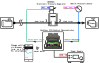
\includegraphics[width=0.90\textwidth]{pic/SchematicHardware.pdf}

    \vfill
    {\large Version \ventconversion\par}
    {\large \today\par}
\end{titlepage}

% ========================== BODY =============================================
\pagenumbering{arabic}

% ---------- SECTION 1: SYSTEM OVERVIEW ---------------------------------------
\section{System Overview}

Unlike a mechanical pressure regulator, which relies on a diaphragm and spring to maintain its setpoint,
the VENTREX electronic pressure regulator uses a software-based feedback control loop.
A PID control algorithm continuously compares the measured outlet pressure with the desired setpoint and modulates the 
proportional valve accordingly.

The VentCon demonstrator showcases this principle: it implements the complete control loop on a microcontroller chip, allowing users to observe and tune the regulator's behaviour in real time.
This document covers the system's hardware, functional principles, and browser-based user interface.


\begin{figure}[H]
    \centering
    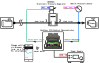
\includegraphics[width=1\textwidth]{pic/SchematicHardware.pdf}
    \caption{VentCon system overview.}
    \label{fig:overview}
\end{figure}

All parameters can be adjusted through a browser-based interface served over WiFi directly from the device. 
No external software, router, or internet connection is required. The VentCon operates fully self-contained, 
making it usable in any environment regardless of existing network infrastructure.

\vfill

\begin{tcolorbox}[
    colback=ventrexblue!8,
    colframe=ventrexblue,
    fonttitle=\bfseries,
    title=Important,
    boxrule=0.6pt,
    arc=2pt
]
The PID control loop runs independently of the WiFi connection.
Even if the browser is closed or the device is disconnected from WiFi, pressure regulation continues uninterrupted 
based on the last applied settings (as long as the power supply remains on). \\[1ex]
This also means that upon switching the power supply on, the system will immediately start to regulate the pressure by 
powering the proportional valve.
\end{tcolorbox}

\pagebreak


% ---------- SECTION 2: GETTING STARTED --------------------------------------
\section{Getting Started}

\subsection{Wiring Scheme}\label{sec:wiring}

The terminal block on the front of the VentCon device (Figure~\ref{fig:terminal}) provides connections for the pressure sensor 
(\texttt{Sen}/\texttt{Sup}/\texttt{GND}), the power supply (\texttt{VIn}/\texttt{GND}) and the proportional valve (\texttt{PV+}/\texttt{PV-}).

\begin{figure}[H]
    \centering
        \includegraphics[width=0.9\linewidth]{pic/Terminal_block.pdf}
        \caption{Terminal block connections.}
        \label{fig:terminal}
\end{figure}
\vspace{-2mm}
The terminal block connections are numbered as follows (from left to right; see Figure~\ref{fig:terminal}).

\vspace{1ex}

The \textbf{Pressure Sensor} (not included in the demo kit) is connected at three positions:
\begin{tcolorbox}[blanker, borderline west={1pt}{0pt}{ventrexblue}, left=1em]

    \begin{enumerate}[leftmargin=6em]
        \item [Pos. \textbf{1)}]\fbox{\texttt{Sen}} Connect this to the analog pressure signal output of the pressure sensor.
        \item [Pos. \textbf{2)}]\fbox{\texttt{Sup}} This connector provides a regulated 5\,V to the pressure sensor. Connect to the 'supply voltage' pin of the pressure sensor.
        \item [Pos. \textbf{3)}]\fbox{\texttt{GND}} Connect to the ground pin of the pressure sensor.
    \end{enumerate}
\end{tcolorbox}

\vspace{1ex}

The \textbf{Power Supply} (not included in the demo kit) is connected at two positions:
\begin{tcolorbox}[blanker, borderline west={1pt}{0pt}{ventrexblue}, left=1em]

    \begin{enumerate}[leftmargin=6em]
            \item [Pos. \textbf{4)}]\fbox{\texttt{VIn}} Connect to the positive terminal of the power supply (red banana plug).
            \item [Pos. \textbf{5)}]\fbox{\texttt{GND}} Connect to the negative terminal of the power supply (black banana plug).
    \end{enumerate}
    \vspace{1ex}
    The power supply must deliver a stable DC voltage. It is used to power the entire system, including the microcontroller, pressure sensor, and proportional valve.
    
    \begin{tcolorbox}[
		colback=ventrexblue!8,
		colframe=ventrexblue,
		fonttitle=\bfseries,
		title=Important,
		boxrule=0.6pt,
		arc=2pt
		]
 		The proportional valve receives the same voltage that is set on the user's power supply.
	\end{tcolorbox}

    For the proportional valve supplied with this demo kit, a 12\,V source rated for at least 4\,A is recommended. The VentCon device, however, accepts any supply voltage in the range of 12 to 30\,V.
\end{tcolorbox}

\vspace{1ex}

Optional external \textbf{Analog Input}:
\begin{tcolorbox}[blanker, borderline west={1pt}{0pt}{ventrexblue}, left=1em]
    \begin{enumerate}[leftmargin=6em]
            \item [Pos. \textbf{6)}] \fbox{\texttt{AI}} Used for external analog input (not used in this demo kit, reserved for future expansion).
    \end{enumerate}
\end{tcolorbox}

\vspace{1ex}

The \textbf{Proportional Valve (PV)} is connected via the provided 2-pin connector (i.e. no user wiring required):

\begin{tcolorbox}[blanker, borderline west={1pt}{0pt}{ventrexblue}, left=1em]
    \begin{tcolorbox}[
        colback=ventrexblue!8,
        colframe=ventrexblue,
        fonttitle=\bfseries,
        title=Important,
        boxrule=0.6pt,
        arc=2pt
    ]
    It is recommended that users first familiarise themselves with sensor behaviour, browser interface, 
    and control parameters before connecting the proportional valve (PV). \underline{See section~\ref{sec:connWifi}.}
    \end{tcolorbox}


    \begin{enumerate}[leftmargin=6em]
            \item [Pos. \textbf{7)}]\fbox{\texttt{PV+}} This is connected to the positive terminal of the proportional valve.
            \item [Pos. \textbf{8)}]\fbox{\texttt{PV-}} This is connected to the negative terminal of the proportional valve.
    \end{enumerate}
\end{tcolorbox}




\subsection{Connecting to the Device via WiFi}\label{sec:connWifi}

It is recommended that before the VentCon device is wired up to the proportional valve, users first connect to the device via WiFi and explore 
the browser interface. The device used for this can be any WiFi-enabled smartphone, tablet or PC with a modern web browser (e.g. Google Chrome, Safari)\footnote{Up to two devices can be connected to the VentCon's WiFi network at the same time.
This allows, for example, a smartphone and a laptop to both access the browser interface simultaneously.}. 

Upon connecting the device to supply voltage, a green indicator LED inside the DEBUG connector on the side of the housing confirms 
that the electronics are successfully powered and the microcontroller is running.
The device will automatically create its own WiFi access point. No router or internet connection is needed or used.
This also means that the device is not able to send or receive any data to or from the internet.

\begin{tcolorbox}[
            colback=ventrexblue!8,
            colframe=ventrexblue,
            fonttitle=\bfseries,
            title=Important,
            boxrule=0.6pt,
            arc=2pt
        ]
    The PID control loop runs independently of the WiFi connection.
    Disconnecting the browser does \emph{not} stop pressure regulation.
\end{tcolorbox}

In order to initiate the connection to the device, follow these steps:

\noindent
\begin{minipage}[ht]{0.4\textwidth}
    \centering
    
\includegraphics[width=0.98\linewidth]{pic/BackSide.pdf}
    \captionof{figure}{QR Code for WiFi connection.}
    \label{fig:backside}
\end{minipage}
\hfill
\begin{minipage}[ht]{0.55\textwidth}
    \vspace{0mm}
        \begin{enumerate}
            \item Power on the VentCon unit via your power supply (connector see Section~\ref{sec:wiring}).
            \item On your smartphone or tablet, scan the QR Code on the back of the device (see Figure~\ref{fig:backside}).
            This will connect to a network called \texttt{VENTCON\_AP}.\\
            Go to step~\ref{item:webinterface} from here.\\[2ex]
            If your device does not support QR code scanning (e.g. on a PC):
            \begin{enumerate}[leftmargin=3em]
                \item[1.] Open WiFi settings on your device.
                \item[2.] Connect to the network \texttt{VENTCON\_AP} using the password \texttt{ventcon12!}
            \end{enumerate}

            \item If your device reports that the network has no internet access, you can safely ignore this notice.\\ 
            VentCon creates a local WiFi network only and does not provide internet connectivity.

            \item\label{item:webinterface} Open a web browser and navigate to\\ \textbf{\url{http://192.168.4.1}} or, alternatively,\\
            \textbf{\url{http://ventcon.local}}
    \end{enumerate}
\end{minipage}%
\vspace{-3ex}
% ---------- SECTION 3: BROWSER INTERFACE ----------------------------------------
\section{Browser Interface}

The browser interface is divided into collapsible sections (tap a header to expand/collapse).
Figure~\ref{fig:browser-app} provides an annotated overview. At the top, real-time status indicators display the current outlet pressure and valve 
duty cycle as gauges. Below, a live trend chart plots the pressure, setpoint and duty cycle over time.
The control parameters section allows adjustment of the pressure setpoint and PID gains ($K_p$, $K_i$, $K_d$). 
Be sure you know the effects of each parameter before making changes (see Section~\ref{sec:pid}).
Additional auxiliary settings, such as the sensor low-pass filter strength, are grouped at the bottom.

A \textbf{Reset PID} button clears the controller's internal state, which is useful when the system is saturated or oscillating.
Finally, a \textbf{Reset to Default} button restores all user-adjustable settings to their factory values after confirmation.

\newpage
\thispagestyle{empty}
\begin{figure}[H]
    \centering
    \vspace*{-\headsep}\vspace*{-\headheight}\vspace*{-\topmargin}\vspace*{-1in}%
    \makebox[\textwidth]{%
        \includegraphics[width=\paperwidth, height=\paperheight, keepaspectratio]{pic/BrowserApp.pdf}%
    }
    \caption{Annotated overview of the VentCon browser application.}
    \label{fig:browser-app}
\end{figure}
\newpage



\subsection{Applying Changes}

Changes are \textbf{not} applied immediately.
After adjusting any parameter, a blue \textbf{Apply Changes} button appears at the bottom of the screen (Figure~\ref{fig:apply}).
Tap it to send all pending changes to the device.
All applied settings are automatically saved to VentCon's flash memory and survive power cycles.

If the \textbf{Apply Changes} button is not tapped within a few seconds, the new settings will \textbf{not} take effect 
and the system will continue operating with the previously applied parameters.

\begin{figure}[H]
    \centering
    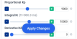
\includegraphics[width=0.4\textwidth]{pic/ApplyButton.pdf}
    \caption{The floating \emph{Apply Changes} button appears when parameters have been modified.}
    \label{fig:apply}
\end{figure}



% ---------- SECTION 4: PID CONTROL BASICS -----------------------------------
\section{PID Control Basics}\label{sec:pid}

Figures~\ref{fig:overview} and~\ref{fig:pid-block} illustrate the closed-loop control architecture.
The pressure sensor continuously measures the outlet pressure (\emph{Process Variable}).
The PID controller computes the error between the \emph{Setpoint} and the measured pressure, and outputs a \emph{Valve Duty Cycle} (PWM signal) to the solenoid valve.

\begin{figure}[H]
    \centering
    \includegraphics[width=0.8\linewidth]{pic/PID_blockDiagram.pdf}
    \caption{PID closed-loop control block diagram.
             The Setpoint is compared with the Outlet Pressure; the error drives
             the Proportional, Integral and Derivative paths whose sum controls
             the Valve Duty Cycle.}
    \label{fig:pid-block}
\end{figure}

The algorithm uses the \emph{Parallel Form} (non-interacting form) of the PID algorithm.
Each control action is computed independently and summed.

\textbf{Proportional} (gain $K_p$): Output proportional to the current error.\\
Higher $K_p$ gives a more aggressive response but can cause overshoot.

\textbf{Integral} (gain $K_i$): Accumulates past error to eliminate steady-state offset.\\
Too high a value causes oscillation (integral windup).

\textbf{Derivative} (gain $K_d$): Damps the response by reacting to the rate of change of the error.\\
Reduces overshoot but amplifies sensor noise if set too high.


\pagebreak

The mathematical representation of the PID controller is given by the following equation:

    \begin{equation*}
    y(t) \;=\; K_p \, e(t) \;+\; K_i \!\int_0^t e(\tau) \, d\tau \;+\; K_d \, \frac{de(t)}{dt}
    \end{equation*}

    \begin{tabular}{rl}
        $y(t)$ & is the controller output (Valve Duty Cycle)\\
        $e(t)$ & is the error (Setpoint\,$-$\,Outlet Pressure)\\
        $K_p$, $K_i$, $K_d$ & are the tunable gains.
    \end{tabular}


    \begin{table}[H]
        \centering
        \begin{tabular}{c|l|l}
        \textbf{Term} & \textbf{Role} & \textbf{Focus} \\ \hline
        $K_p$  & Present & Reacts to \emph{how far} you are from target \\
        $K_i$  & Past    & Reacts to \emph{how long} you have been away \\
        $K_d$  & Future  & Reacts to \emph{how fast} you are approaching/leaving
        \end{tabular}
        \caption{PID term summary.}
    \end{table}






% ---------- SECTION: TUNING GUIDE -----------------------------------------
\subsection{Tuning Guide}

Follow these steps for initial tuning. Observe the \textbf{Live Chart} after each change.

\begin{enumerate}
    \item \textbf{Set a Stable Operating Point.}
          Choose a moderate setpoint (e.g.\ 6\,bar(g)), let the system settle.

    \item \textbf{Start with P-only control.}
          Set $K_i = 0$ and $K_d = 0$.
          Begin with a low $K_p$ and increase gradually.
          Find the value where the pressure just begins to oscillate steadily (\emph{ultimate gain}), then back off slightly.

    \item \textbf{Introduce Integral action.}
          Slowly increase $K_i$ to remove the remaining steady-state offset.
          Stop increasing when further gains cause oscillation.

    \item \textbf{Add Derivative action (if needed).}
          If the response overshoots or is slow to settle, increase $K_d$ cautiously to add damping.

    \item \textbf{Iterate.}
          Make small single-parameter changes and observe.
          The goal is a fast, smooth response with minimal overshoot.
\end{enumerate}

\subsection{Example: Step Response}

Figure~\ref{fig:step} shows a typical step-response recording where the setpoint is changed from 4 to 6\,bar.
Figure~\ref{fig:disturbance} demonstrates the controller rejecting a mass-flow disturbance while maintaining the setpoint.

\begin{figure}[H]
    \centering
    \begin{minipage}[t]{0.48\textwidth}
        \centering
        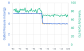
\includegraphics[width=\linewidth]{pic/Example_Set_4_to_6_bar.pdf}
        \caption{Setpoint step from 6 to 4\,bar.}
        \label{fig:step}
    \end{minipage}\hfill
    \begin{minipage}[t]{0.48\textwidth}
        \centering
        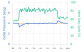
\includegraphics[width=\linewidth]{pic/Example_Regulator_Action_Massflow_Variation.pdf}
        \caption{Disturbance rejection under varying mass flow.}
        \label{fig:disturbance}
    \end{minipage}
\end{figure}

% \begin{figure}[H]
%     \centering
%     \includegraphics[width=0.3\linewidth]{pic/Where the hands work, there Lakshmi resides.pdf}
%     \label{fig:bestwishes}
% \end{figure}

\end{document}